\documentclass[12pt]{article}
\usepackage{graphicx}
\usepackage {color}
\usepackage{pdfpages}
\usepackage{float}
\usepackage{changebar}
\usepackage{enumitem,amssymb}
\renewcommand{\familydefault}{\sfdefault}
\usepackage[margin=1.2in]{geometry}
\usepackage{graphicx}
\usepackage{wrapfig}
\usepackage[super]{cite}
\usepackage{subcaption}
\usepackage[table]{xcolor}
\usepackage{amsmath}
\usepackage[sort, numbers]{natbib}
\usepackage{multirow}
\usepackage{tabularx}
\usepackage{siunitx}

%%%%%%%%%%%%Defining the margins %%%%%%%%%%%%%%%%%%%%%
\textheight 9.in
\textwidth 6.5in
\topmargin -.5in
\oddsidemargin 0in
\setlength{\parskip}{\smallskipamount}

%%%%%%%%%%%%%%Specific Commands %%%%%%%%%%%%%%%%%%
\newcommand{\eg}{{\em e.g.,}}
\newcommand{\ie}{{\em i.e.,}}
\newcommand{\etc}{{\em etc.,}}
\newcommand{\etal}{{\em et al.}}
\newcommand{\degrees}{{$^{\circ}$}}
\newcommand{\fig}[1]{\textbf{Figure #1}}
\DeclareMathOperator*{\argmin}{argmin}
%%%%%%%%%%%%%%%%%%%%%%%%%%%% Setting to control figure placement
% These determine the rules used to place floating objects like figures 
% They are only guides, but read the manual to see the effect of each.
\renewcommand{\topfraction}{.9}
\renewcommand{\bottomfraction}{.9}
\renewcommand{\textfraction}{.1}
\renewcommand{\familydefault}{\sfdefault} %setting the san serif font

%%%%%%%%%%%%%%%%%%%%%%%% Line spacing
% Use the following command for ``double'' spacing
%\setlength{\baselineskip}{1.2\baselineskip}
% and this one for an acceptable NIH spacing of 6lpi based on 11pt
%\setlength{\baselineskip}{.9\baselineskip}
% The baselineskip does not appear to work when we include a maketitle
% command in the main file.  Something there must set the line spacing
% If we use this next command, then things seem to work.
\renewcommand{\baselinestretch}{.9}
\newcommand{\rpm}{\raisebox{.2ex}{$\scriptstyle\pm$}}
\setcounter{secnumdepth}{0} %make no numbers but have a table of contents


\begin{document}
	
	\title{Troponin-C }
	\author{Jake Bergquist, u6010393 }
	\maketitle
	
	\section{Abstract}
	Troponin-C is a calcium binding protein that acts to regulate the interface between the calcium cycles within myocytes and the subsequent muscle fiber contraction as a part of the troponin complex. This key regulatory role links the calcium cycle and contraction of muscles, and this protein is implicated in several disease states such as certain types of cardic myopathy. Troponin-c is found bound to the troponin complex in cardic and skeletal muscles and can be extracted via ethanpol precipitation and chromatography from muscle samples. It is a single polypeptide, primarily alpha-helix protein with two main domains, each of which having two calcium binding sites. 
	
	\section{Introduction}
	Troponin-C is a protein found in skeletal and cardiac muscle that helps control the initiation of contraction of the muscle fiber.\cite{Li2015} Troponin-C is one of many proteins in a  regulatory complex of troponin proteins (troponin 1, C and L) which all act to modulate the binding of tropomyosin to actin filaments in the muscle. The function of the troponin complex, and by extension the function of troponin-c, is critical to the proper timing, strength, and frequency of muscle contraction in both skeletal and cardiac muscle.\cite{Li2015} Troponin is also used as a biochemical marker of heart health during potential instances of acute cardiac damage such as a myocardial infarction, as it is released into the blood when cardiomyocytes are damaged.\cite{Melanson2007} Troponin-C is a type of calcium binding protein with two distinct conformations that are stabilized by different concentrations of calcium.\cite{Strasburg1980,Rao1996,Greaser1973} This allows troponin C to regulate muscle contraction (in conjunction with the rest of the troponin/tropomyosin complex) in a calcium dependent manner. Changes to troponin-C are implicated in several disease processes, particularly of cardiac troponin-C which plays a role in some forms of cardiomyopathy. Several pharmacological treatments of this disease state target troponin-C specifically.\cite{Melanson2007} Troponin-c is the key link between myocyte calcium concentration (which rises in response to contraction stimulus) and the initiation and maintenance of muscle contraction.\cite{Li2015} Without this link there would be no whay for seleltal muscle to contract when stimulated by motor neurons, and there would be no way for cardiac myocytes to contract in response to waves of action potentials through the heart. Missfunction (calcium sensitivity changes and regulatory effect/binding chages) can also have pathophysiological consequences.\cite{Li2015} Thus this protein is critical not only for voluntary movement of skeletal muscle but also critical functions such as heart contraction.
	
	\subsection{Structure and Function}
	
	\begin{figure}[H]
		\centering
		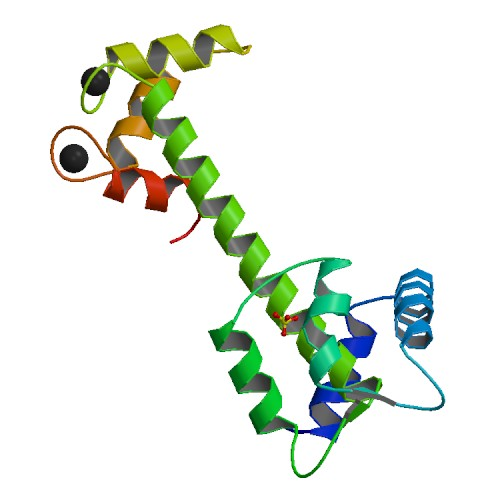
\includegraphics[width=.55\linewidth]{ncx.png}
		
		\caption{Ribbon diagram for 1NCX Troponin-C\cite{Rao1996}}
		\label{struct}
	\end{figure}
	
	Troponin-C is a 18 KDa  protein of the EF-hand family of calcium binding proteins.\cite{Rao1996} There are several variants of this structure depending on the type of muscle it is found in, but all play a similar role in the regulation of calcium induced contraction of muscle fibers. Generally troponin-C is composed of two main domains, each with two calcium binding EF-hand motifs.\cite{Rao1996,Leavis1978} The two domains are connected by a flexible linker region with a dynamic structure in solution. Troponin-C exists in two main conformational shapes, open and closed, and the transition is dictated by the binding of calcium ions to the calcium binding motifs. Calcium binding drives the protein towards the open confirmation in which a ``sticky" hydrophobic region becomes exposed. This hydrophobic region then binds to the regulatory switch region of troponin-I, removing an adjacent inhibitory region of troponin-1 from its binding site on actin.\cite{Li2015} The now free actin can participate in the binding cycle associated with contraction of the sacomere, and thus the muscle fiber as a whole. Falling calcium ocncentrations (cuased by calcium uptake into the sarcoplasmic reticulum and eflux from the cell via pumps) causes troponin-C to unbind and return to its closed conformation, allowing troponin-1 to rebind to actin inhibiting further contraction.\cite{Bers2002,GDLamb;Society2000} This entire function is mainly driven by two of the four calcium binding domains which are calcium selective. The other two domains can bind magnesium as well as calcium and are thought to play a part in formation of the troponin regulatory complex.\cite{Li2015}
	
	\subsection{Homology and Structural Similarity}
	Trponin-C itself has homologs in all cardiac and skeletal muscle, usually denoted as cardiac troponin-C (c-Tnc) and skeletal troponin-c (s-Tnc). As a member of the EF calcium binding domain troponin-c has homologous calcium binding sites (called EF-hands) to a wide variety of calcium binding proteins such as calmodulin. The EF binding domain is the most common calcium binding motif found in proteins and is used for calcium buffering, signal transduction and regulatory functions.\cite{Lewit-Bentley2000} The EF hand is a helix-loop-helix motif with usually 12 residues makign up the metal coordinating binding site. The binding site can usually accomodate either magnesium or calcium, with an octahedron coordinating geometry for magnesium, and a pentagonal bipyramidal structure coordinating calcium.\cite{Lewit-Bentley2000}
	
	\subsection{Isolation and Purification}
	Troponin-C can be isolated and purified using a series of precipitation assays followed by cation then anion exchange chromatography.\cite{Greaser1973,Greaser1971,Strasburg1980} The primary source of troponin-c used experimentally is muscle tissue samples. Tissue is extracted, washed, pulverized, and the proteins are extracted using ethanol extraction.\cite{Greaser1973,Greaser1971,Strasburg1980} Cardiac troponin complex (including c-Tnc) have a unique N-terminal amino acid sequence that can be used for detection in blood via antibody assays. This is a useful clinical diagnostic marker of cardiac damage as damaged cardiac myocytes release troponin into the blood during adverse cardiac events such as a heart attack. For this reason, troponin assays designed to identify cardiac troponin by this n-terminal sequence, are a common lab work done for patients in whom cardiac events are suspected.\cite{Melanson2007}
	
	\section{Solution Studies}
	The calcium or other divalent ions (usually magnesium 2+) plays a key role in the stability of the calcium binding domains of troponin-c, and the protein as a whole. It has been found that in the absence of these ions the melting point of the binding domains falls from over 90\degrees Celsius to 50\degrees Celsius.\cite{Brzeska1983} Troponin-C is always bound to the troponin complex at actin binding sites in muscle tissue, and because of that it does not diffuse through the cell, thus the diffusion coefficient for troponin-c is not characterized.
	
	\section{Interfacial Studies}
	The four calcium binding sites of troponin-c are split between two lower affinity calcium specific binding sites, and two higher affinity calcium binding sites for which magnesium binds competitively. The binding of calcium to the lower affinity sites causes a conformational change associated with increased alpha helix content and is accompanied by an increased flourescence in the 200 to 240 nm range.\cite{Leavis1978} This conformational change is associated with the regulatory activity of troponin-c. The binding affinities of troponin-c cannot be explained by any of the subunits in isolation and is rather a consequence of interaction between the different subunits. The nature of this cooperative binding is not fully understood.\cite{Leavis1978}
	
	\section{Predictions}
	Using the structure and primary sequence of troponin-C (1NCX on RSCB) the following structure and chemical property predictions can be made. Based on the amino acid sequence the secondary structure predictions shown in Figure~\ref{secondStruct} shows a large degree of alpha helix content within the secondary structure. This prediction agrees well with the solved crystal structure which also contains a large number of helical segments. There are some inconsistencies between the predictions and the measured secondary structure, such as leu 14 and ser 15 are predicted to be in an alpha helix but are not in the solved structure. Despite this the prediction is largely accurate for this protein.
	
	\begin{figure}[H]
		\centering
		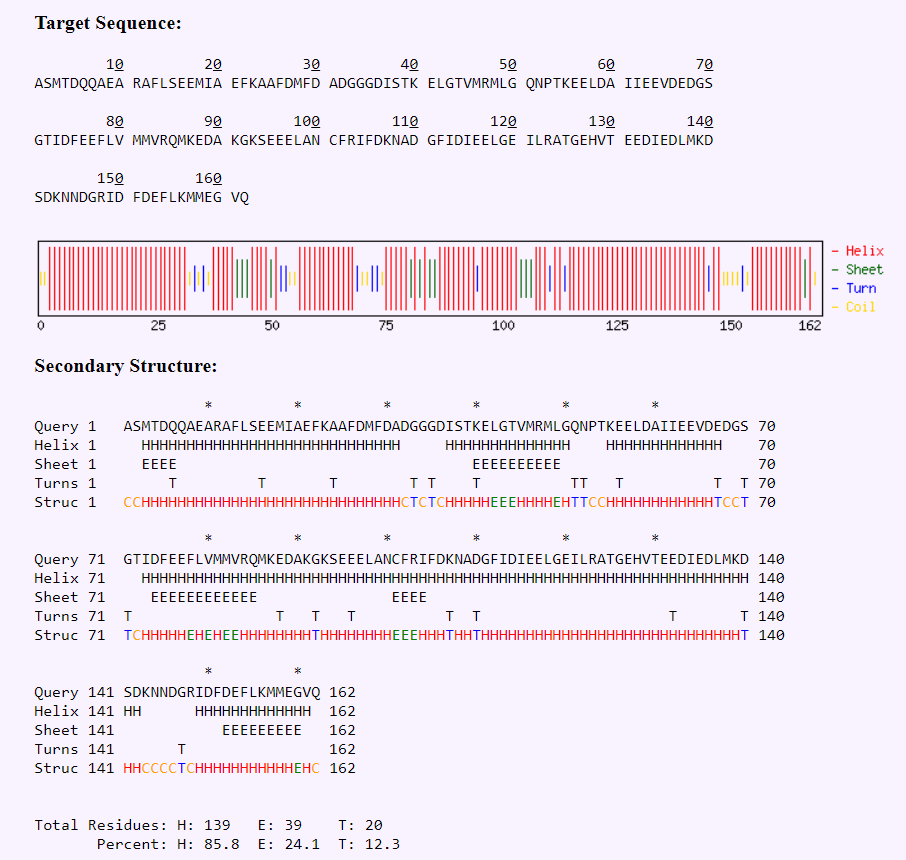
\includegraphics[width=.95\linewidth]{SecondaryStructureAnalysisPlot.png}
		
		\caption{Predicted secondary structures based on sequence.}
		\label{secondStruct}
	\end{figure}
	
	Using the first predicted helix from the secondary structure prediction (Figure~\ref{secondStruct}) the calculated amphiphilicity is shown in Figure~\ref{helix1}. As can be seen there is fairly ordered arrangement across the helix with most of the polar residues on one side and most of the non-polar on the other. This results in a hydrophobic moment of $0.251 \mu H$ and a hydrophobicity of $0.325 H$.
	
	\begin{figure}[H]
		\centering
		\includegraphics[width=.95\linewidth]{Helix1_plot.png}
		
		\caption{Helix amphihilicity predictions based on the sequence of the first major helix from the secondary structure predictions in Figure~\ref{secondStruct}}
		\label{helix1}
	\end{figure}
	
	A titration prediction the isoelectric point at 4.13 (Figure~\ref{titration}). At physiologic pHs the charge of the protein is predicted to be in the -20 to -30 range with a charge of -22 at a pH of 6.5.
	
	\begin{figure}[H]
		\centering
		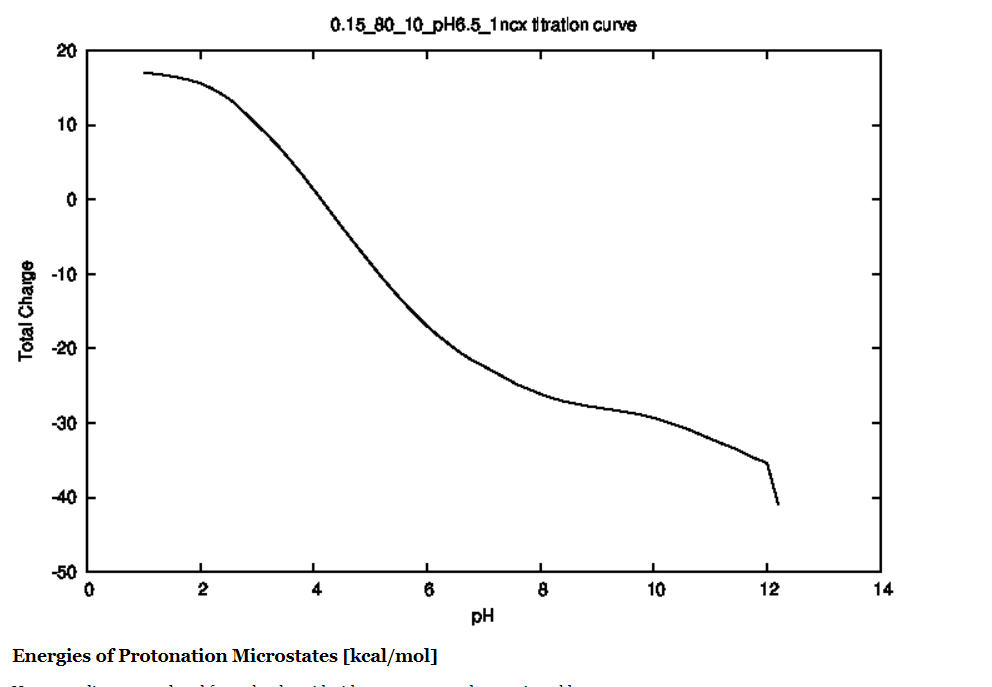
\includegraphics[width=.75\linewidth]{ComputedTitration.png}
		
		\caption{Predicted titration curve of troponin-C. The isoelectric point is 4.13.}
		\label{titration}
	\end{figure}
	
	A hydrophobic cluster analysis (Figure~\ref{hca}) shows the environments around each of the amino acids. As can be seen there tend to be glycene (diamonds) near to the hydrophobic clusters (green). There is no signlar hydroiphobic core but rather several groups spread throughout the sequence. This may be related to the aphipathic character predicted in Figure~\ref{helix1} as the hydrophobic residues are arranged on one side of a helix.
	\begin{figure}[H]
		\centering
		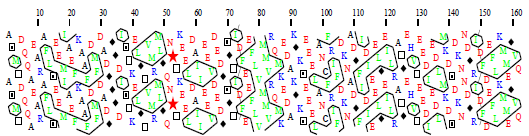
\includegraphics[width=\linewidth]{HCA.png}
		
		\caption{Calculated Ramachandran plot according to structure.}
		\label{hca}
	\end{figure}
	
	Using the solved structure the ramachandran plots shown in Figure~\ref{ramchan} are produced. In the generic plot we see that most of the amino acids predictably fall into the alpha helix region of the plot rater tightly. This is expected given the high alpha helical content of troponin-c. There are also several residues in the beta sheet region. However, there is very little actual beta sheet structure in troponin-c meaning that some regions may be in a conformation that would be permissible for beta sheet formation, but there are not neighboring amino acids such that a beta sheet would be formed. There are no trans-proline structures and only one cis proline which falls well within a stable region. Only one residue, Ala-31, is outside of a stable region, although it is not far off.
	
	
	\begin{figure}[h]
		\centering
		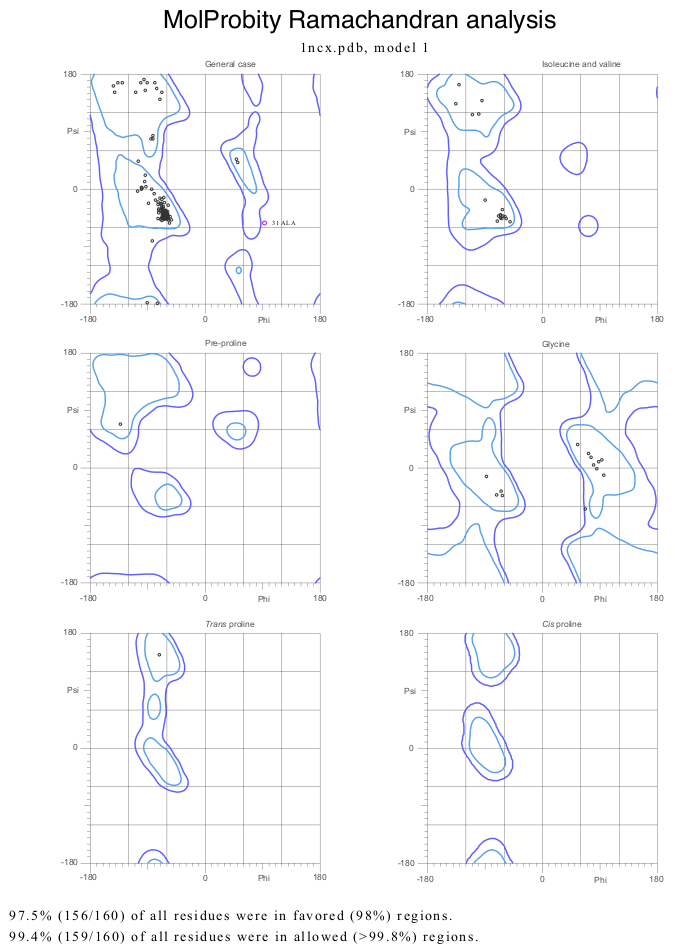
\includegraphics[width=.75\linewidth]{ramachandran.png}
		
		\caption{Calculated ramachandran plot based on structure for general case, isoleucine-valine, pre-proline, glycine, trans-proline, and cis-proline.}
		\label{ramchan}
	\end{figure}
	\section{Calculations}
	
	Using python molecular viewer the electrostatic potentials in low (0.01 M) and high (0.15 M) monovalent ionic solutions are found to be $3.00*10^4 kJ/mol$ and $2.99*10^4 kJ/mol$ respectively. It is interesting to note a very minimal difference in energy between the two solutions. In order to calculate the hydration and solvation energies first the free energy at a solution dielectric equal to the protein interior dielectric (dielectric of 2, 0 M salt solution) is calculate to be $5.31 *10^4 kJ/mol$. Next, for hydration the free energy in water is calculated to be $3.00*10^4$ with a solution dielectric constant of 78.5 (0.01 M salt solution). Subtracting the free energy in water from the free energy in protein solution we get the energy of hydration of $2.31*10^4 kJ/mol$. Using a similar process the energy of solvation is calculated. First the free energy in a vacuum (dielectric of solution set to 1, 0M salt solution) is calculated ($7.00*10^4kJ/mol$) and subtracted from the free energy in water($3.00*10^4$). This yields the solvation energy of $4.00*10^4kJ/mol$.
	
	Using the calculated fraction of area exposed and the known hydrophobicities and hydrophilicities the total protein hydrophobicity and hydrophilicites can be calculated. This is done by summing the hydrophobicity for each side chain multiplied by its percent of exposure (the percent of its total area exposed to solution). This yields a hydrophobicity of $1.40*10^3 kJ/mol$, and a hydrophilicity of $-2.40*10^3 kJ/mol$. This demonstrates that troponin-c is highly hydrophilic, as would be expected given its environment in the cell is surrounded by aqueous solution in which its calcium binding domains can detect changes in calcium concentration.
	%Solvation energy Ginitial = 6.995327002832E+04 kJ/mol (in: 2, out:0, soul: 0 M)
	%Solvation energy Gfinal = 3.003811168637E+04 kJ/mol (in: 2, out: 78.5 0.01 M)
	
	%Hydration energy Ginitial = 5.305483322598E+04 kJ/mol (in:2, out:2, soul 0 M)
	%Hydration energy Gfinal = 3.003811168637E+04 kJ/mol (in: 2, out: 78.5 0.01 M)
	
	%high ionic strength G =2.992309508231E+04 kJ/mol (in:2 out:78.5, 0.15 M)
	%low ionic strength G = 3.003811168637E+04 kJ/mol (in: 2, out: 78.5 0.01 M)
	
	
	%Hydrophobicity: 1298.2 kJ/mol
	%Hydrophilicity: -2394.7 kJ/mol
	\section{Conclusion}
	Troponin-c is a vital regulator of myosin driven muscle contraction in both cardiac and skeletal muscle. Improper function fo this protein leads to a breakdown of the calcium signaling triggered contraction of muscles. Ata skeletal muscle level this leads to a reduced or complete loss of control of muscle function. For the cardiac muscle this leads to a disconnect between the myocardial action potentials and the myocardial contraction, leading to heart contraction failure and death. Damage to muscle causes release of the troponin complex, which contains troponin-c, into the blood stream. Because cardiac troponin can be differentiated from others this makes it an ideal biomarker for diagnostics of heart damage such as what might occur during a heart attack. Troponin-c is the linking point between intracellular calcium concentration change and muscle contraction via its calcium binding domains which initiate a regulatory cascade that allows for myosin binding to actin and subsequent contraction.
	
	\bibliography{D:/Users/Jake/Documents/library}
	\bibliographystyle{IEEEtran}
	
	
\end{document}

















